\appendix
\section{Appendix}\label{sec:appendix}
\subsection{Team contributions}\label{appendix:team_contributions}
\begin{itemize}
    \item \textbf{Niko:} setup of local server, minimax player, $\alpha$-$\beta$ pruning and heuristics.
    \item \textbf{Giuseppe:} gimmick rules, $\alpha$-$\beta$ pruning, heuristics and scripts for running the players.
    \item \textbf{Alessandro:} stats and damage computation, baseline players, matchup rules and rule-based player.
\end{itemize}

\subsection{Github metrics}\label{appendix:github_metrics}
\begin{table}[!htbp]
    \footnotesize
    \centering
    \begin{tabular}{c|c|c}
        \hline \hline
         \textbf{Member} & \textbf{Commits} & \textbf{Major activity period} \\ \hline \hline
         Niko & 55 & middle of november \\ \hline
         Giuseppe & 37 & middle of november \\ \hline
         Alessandro & 57 & start of november \\ \hline \hline
    \end{tabular}
    \caption{Github contributions for each member}
    \label{tab:git_contributions}
\end{table}

\subsection{Relationship with the course}\label{appendix:course_relationship}
\begin{itemize}
    \item Study and definition of the problem:
    \begin{itemize}
        \item Definition of the environment and its characteristics.
        \item Definition of the type of game.
        \item Acting under uncertainty.
    \end{itemize}
    \item Definition of the agents:
    \begin{itemize}
        \item Logical agent (Rule-based)
            \begin{itemize}
            \item Definition of rules in FOL.
            \end{itemize}
        \item MiniMax algorithm
            \begin{itemize}
            \item $\alpha$-$\beta$ pruning.
            \item Definition of the Heuristic function.
            \end{itemize}
    \end{itemize}
    \item Exploit non-cooperative Game Theory:
    \begin{itemize}
        \item Weak dominant strategy for type matchup.
    \end{itemize}
    
\end{itemize}

\subsection{Mini-max tree}
\begin{figure}[H]
    \centering
    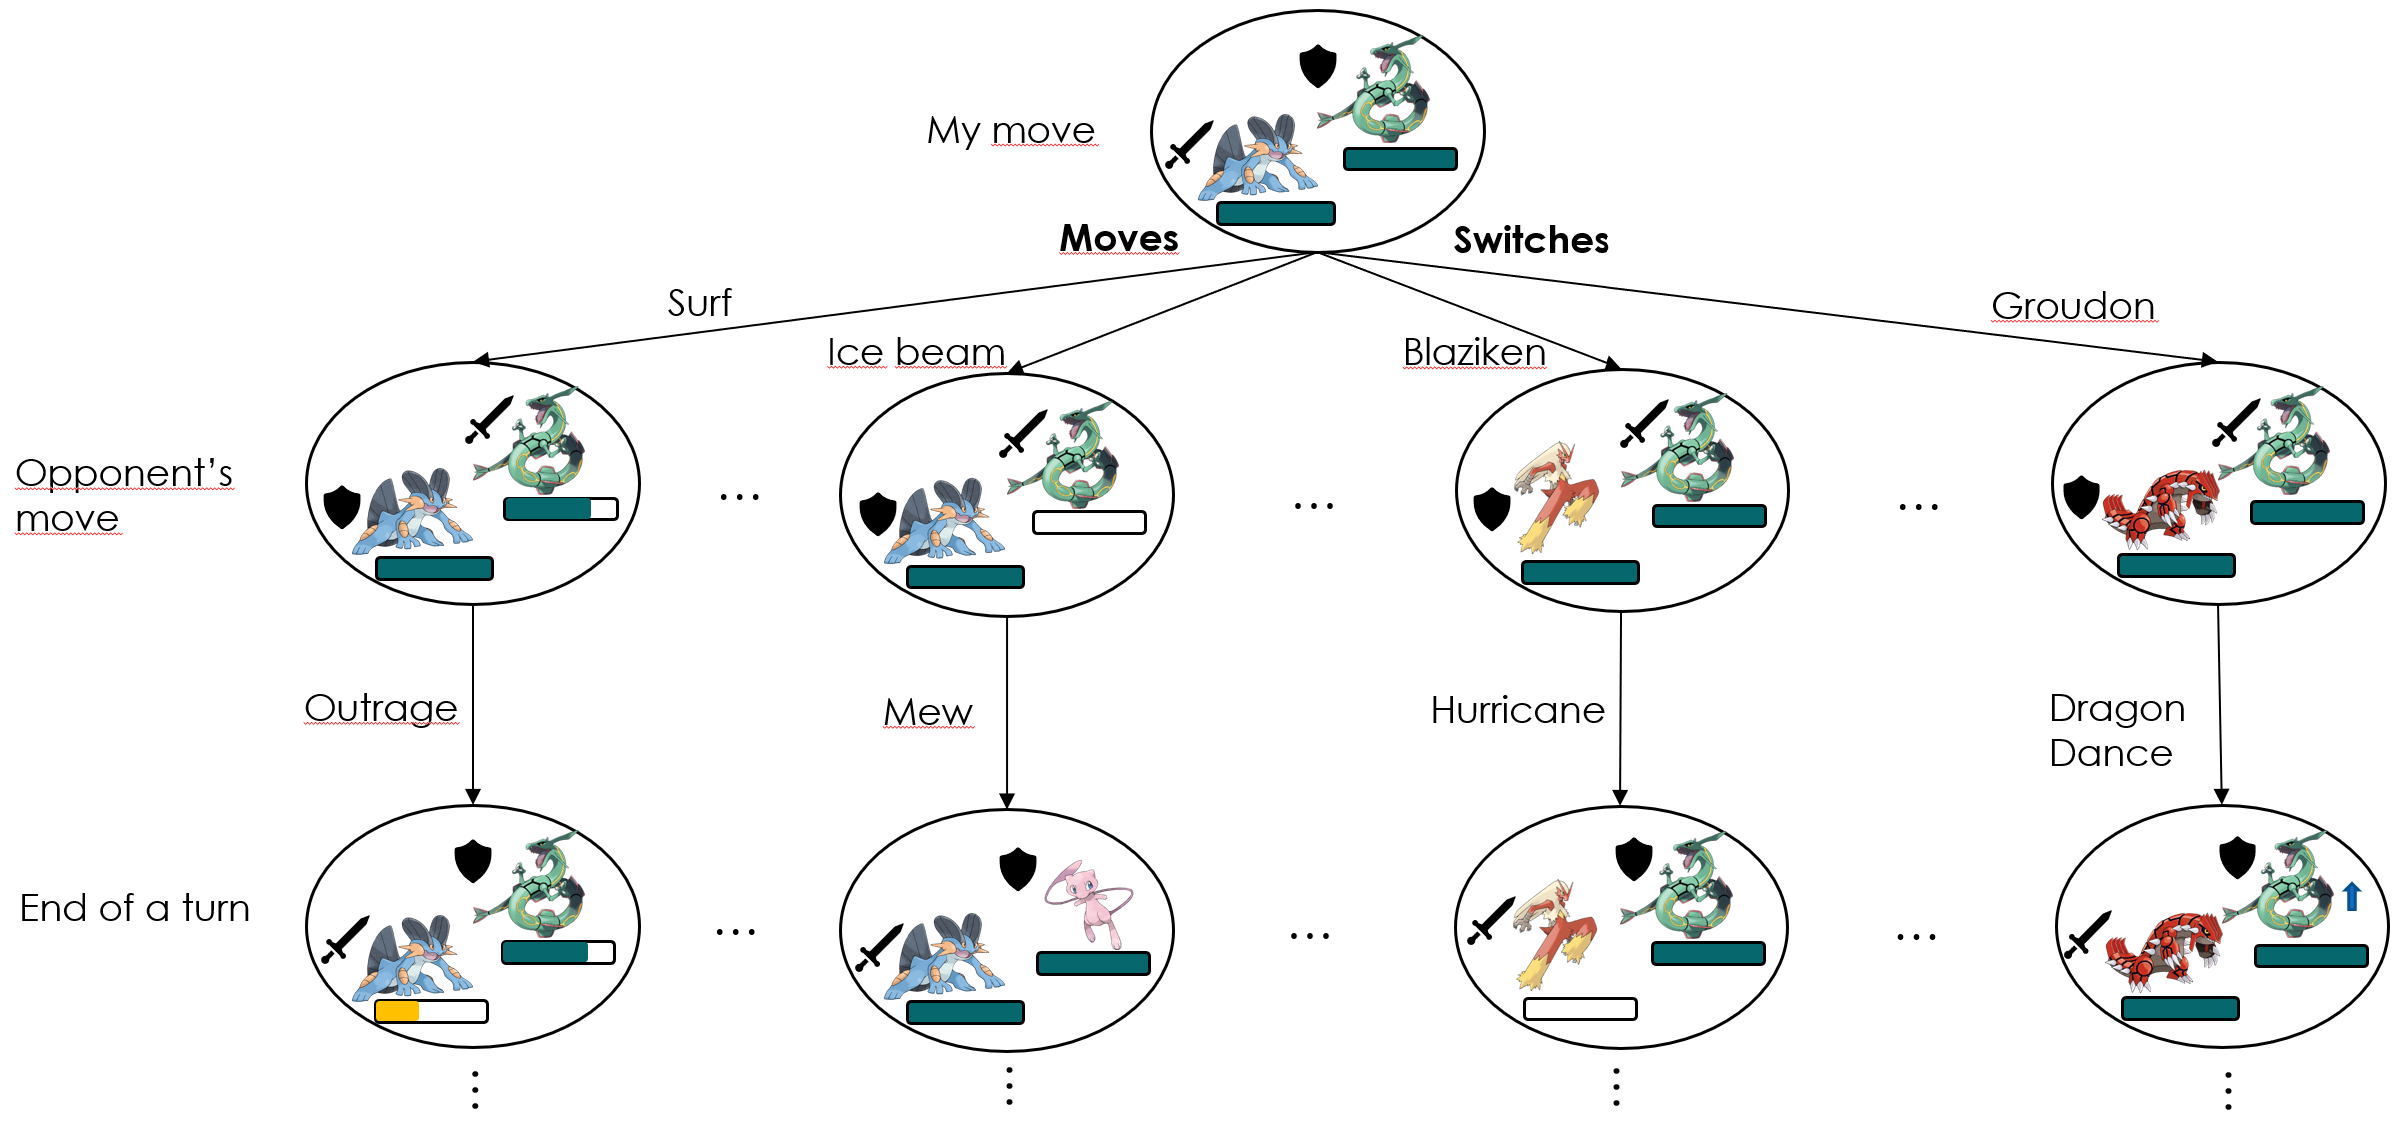
\includegraphics[width=0.8\textwidth]{images/minimax with switches.png}
    \caption{Minimax tree with switches.}
    \label{fig:minimax_with_switches}
\end{figure}

\begin{figure}[H]
    \centering
    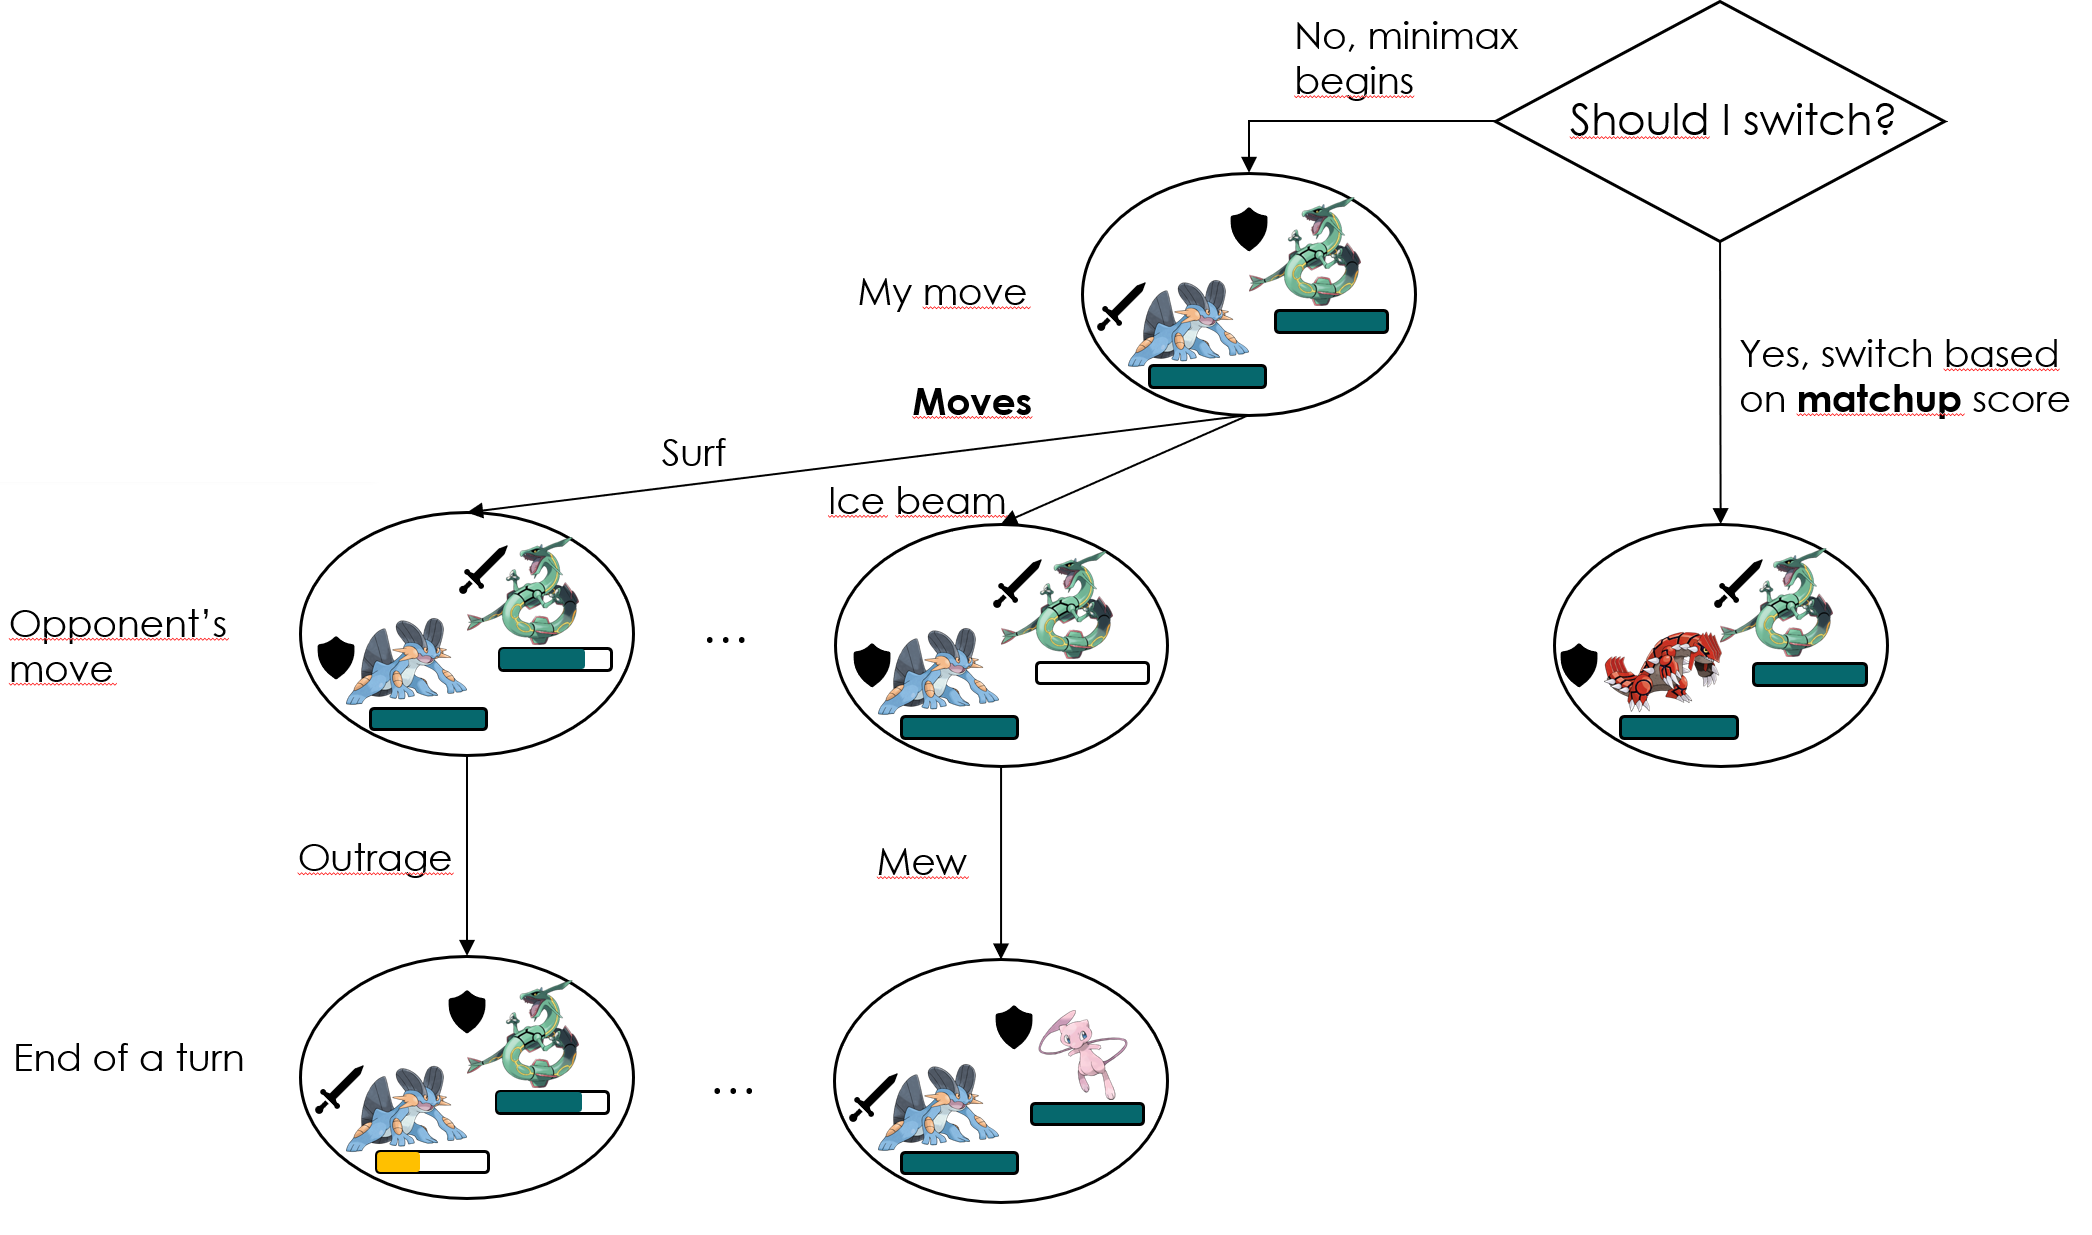
\includegraphics[width=0.8\textwidth]{images/minimax no switches.png}
    \caption{Minimax tree without switches.}
    \label{fig:minimax_without_switches}
\end{figure}
